\documentclass[10pt]{article}
\usepackage{url,hyperref}
%\usepackage{times}
\usepackage[left=1in,right=1in,top=1in,bottom=1in]{geometry}
\usepackage[utf8]{inputenc}
\usepackage{amsmath, xparse}
\usepackage{graphicx}
\graphicspath{ {./images/} }

\begin{document}

\noindent \textbf{CAP 6640 -- Natural Language Processing\hspace*{\fill}Spring 2025}\\
\noindent{\bf Homework \#5} \hfill Due date: March 13, 2025

%\vspace*{-0.1in}\paragraph{Instructions:}
%Individual work. Cite all references. All submitted assignments must be typed. Using Latex is required. For \LaTeX, you may use your installation, or online IDEs (no installation required); e.g.,  \href{https://www.overleaf.com/}{www.overleaf.com}. Late submissions by at most 24 hours will be scaled down to 50\%; late beyond 24 hours will be worth 0\%. Total of 40 points. 

\begin{description}
\item[Problem 1:]  \hfill %List and explain four methods for model comparison in natural language processing.

\begin{enumerate}
    %\item \textbf{Perplexity (PPL):} PPL is a measure of how well a probability distribution or language model predicts a sample. 
    %It is calculated as the inverse probability of the test set, normalized by the number of words.
    %
    %\begin{center}
    %    $\displaystyle{PPL(W) = 2^{(-\frac{1}{N}\sum{log_2{P(w_i)}})}}$
    %\end{center}
    %
    %where $N$ is the number of words in the test set, and $P(w_i)$ is the probability assigned to the $i$-th word by the language model.
    %
    %Lower PPl values indicate better performance. It is a widely used metric for evaluating probabilistic language models like RNNs, LSTMs, and transformers.

    \item \textbf{Bilingual Evaluation Understudy (BLEU):} BLEU is a measure of the accuracy of machine-translated text by comparing it to one or more human references by calculating
    n-gram precision or n-gram overlap between each other. Higher BLEU scores indicate better translation quality like the actual human text.
    It is commonly used metric in machine translation, text generation, and summarization tasks.
    
    \item \textbf{Recall-Oriented Understudy for Gisting Evaluation (ROUGE):} ROUGE is a measure of recall-based text similarity between machine-generated summaries and human references.
    There are two types of ROUGE scores: ROUGE-N, which measures n-gram overlap with the following formula:

    \begin{center}
        $\displaystyle{ROUGE-N = \frac{\sum_{matched\ n-grams}}{\sum_{reference\ n-grams}}}$
    \end{center}
    
    ROUGE-L, which measures how well the longest subsequence matches between reference and generated text.
    It is commonly used in text summarization tasks to evaluate the quality of generated summaries.
    
    \item \textbf{Metric for Evaluation of Translation with Explicit Ordering (METEOR):} METEOR is a translation evaluation metric improving on BLEU by considering 
    exact match, stemming, synonyms, along with precision, recall, and fragmentation penalties. Compared to BLEU, it reveals higher relationships especially with the 
    involvement of human judgements. It is used to evaluate the quality of machine-translated text and paraphrase.
    
    \item \textbf{BERTScore:} BERTScore uses pretrained BERT embeddings to measure similarity between generated and reference texts, capturing semantic 
    meaning rather than just n-gram overlap. It is mostly used for complex NLP assessments like translation, summarization, and dialogue understanding.

\end{enumerate}

\pagebreak

\item[Problem 2:]  \hfill %Differentiate between vertical and horizontal gating.

Gating mechanisms in NNs control the flow of information by selectively allowing or blocking certain values. 
Vertical and horizontal gating are two approaches used to regulate information within deep learning architectures.

\begin{enumerate}
    \item \textbf{Horizontal Gating:} Horizontal gating regulates information flow across time steps in sequential models such as RNNs,
    LSTMs, and GRUs. It helps models retain or discard past information at each time step, making it essential for handling long-term dependencies in sequential data.
    A key example is the forget gate in LSTMs, which determines how much past information should be kept using the formula $f_t = \sigma(W_f h_{t-1} + U_f x_t + b_f)$.
    Horizontal gating is crucial in machine translation, speech recognition, and NLP tasks, where preserving context over time is necessary. 
    However, training these models on very long sequences can be challenging, sometimes requiring attention mechanisms to improve performance.

    \item \textbf{Vertical Gating:} Vertical gating controls information flow across layers in deep neural networks, such as CNNs and ResNets, 
    helping regulate how much information passes from one layer to the next. 
    It is commonly used in Highway Networks and ResNets, where gates determine whether an input is transformed or passed directly to the next layer,
    aiding in gradient flow and feature learning. A key example is the Highway Network, where the transform gate $T(x)$ modulates the proportion of tranformed information
    versus unchanged input using the formula $y = T(x) \cdot H(x) + (1 - T(x)) \cdot x$. Vertical gating is particularly useful in deep architectures to prevent vanishing 
    gradients, making it effective for image classification and other deep learning tasks. However, it does not model temporal dependencies, as it only functions across 
    layers, not time steps.
    
\end{enumerate}

\pagebreak

\item[Problem 3:]  \hfill %Describe how batch normalization improves NLP model performance.

Batch normalization is a widely used technique for CNNs to improve training stability and efficiency.
It works by normalizing activations across a batch, ensuring that NN outputs have zero mean and unit variance, 
which helps to prevent extreme activations that could slow down learning. 
Additionally, batch normalization includes trainable scale $\gamma$ and shift $\beta$  parameters, 
allowing the model to adjust the normalization dynamically rather than simply standardizing all activations.

One of the main advantages of batch normalization is that it reduces internal covariate shift, 
a problem where changing distributions of activations across layers make training less stable. 
By normalizing inputs before they are passed to the next layer, batch normalization ensures that each layer receives consistently scaled data, 
reducing the burden on later layers to adapt to distributional shifts. This leads to faster and more stable training.
Furthermore, it also mitigates vanishing and exploding gradient problems, which commonly occur in deep networks. 
By keeping activations within a reasonable range, it prevents gradients from shrinking too much or growing uncontrollably, 
which can significantly slow down or disrupt training. In addition, it makes parameter initialization less critical, 
since it automatically rescales outputs, reducing the need for carefully chosen weight initializations.
Lastly benefit is that it allows higher learning rates without causing instability, making hyperparameter tuning more forgiving. 
Typically, deep NLP models require very small learning rates to avoid divergence, but batch normalization stabilizes activations, 
enabling the use of more aggressive learning rates that speed up convergence.

\pagebreak

\item[Problem 4:]  \hfill %Explain how very deep CNNs process text.

Traditionally, sequence models like LSTMs and GRUs have dominated NLP due to their ability to handle sequential dependencies. 
However, very deep CNNs which are inspired by image-processing architectures like VGG can be highly effective for NLP, 
particularly in text classification tasks.

Instead of relying on word embeddings and sequential processing, very deep CNNs extract features directly from character-level representations. 
The model consists of multiple stacked convolutional layers, which progressively refine text representations, much like deep CNNs do for images. 
The deeper the network, the more hierarchical and abstract the extracted linguistic features become.

Very deep CNNs apply multiple convolutional layers, followed by pooling layers, to extract patterns in text at various levels. 
This process is similar to how deep CNNs for vision detect simple edges in early layers and complex objects in deeper layers. 
In NLP, this results in low-level character n-grams at shallow layers and high-level semantic representations at deeper layers.
Local pooling at each stage reduces the temporal resolution while retaining key information.
Stacking convolutional layers enables multi-scale text representation, allowing the model to capture both local and long-range dependencies.
This fully convolutional architectures allows for parallel processing, significantly speeding up training.
Deeper CNN architecture improves feature extraction, making the model more effective at capturing linguistic structures.
By leveraging hierarchical feature learning, very deep CNNs can outperform sequence models in text classification tasks, especially when trained on large datasets.

\pagebreak

\item[Problem 5:]  \hfill %Describe how QRNNs work conceptually and mathematically, including their purpose and a supporting figure.

RNNs are effective at capturing sequential dependencies, but they suffer from slow training times due to their sequential nature, 
where each time step depends on the previous one. Quasi-Recurrent Neural Networks, or QRNNs in short, offer a solution by combining the strengths of RNNs and CNNs.
QRNNs use convolutions to capture local dependencies in parallel, similar to CNNs, while gated pooling operations retain long-term dependencies like RNNs.

QRNNs replace the recurrent computations in standard RNNs with 1D convolutions followed by pooling, allowing parallelized sequence processing. 
This is done in two steps. In the first step, QRNNs first apply a 1D convolution over the input sequence to extract features in parallel as

\begin{center}
    $Z_t = $ Conv1D$(X_t, W)$ 
\end{center}

where $X_t$ is the input at time step $t$, $W$ is the convolutional filter, and $Z_t$ is the output feature map. 
Unlike RNNs, which update one state at a time, QRNNs process all time steps simultaneously using convolutional filters. 
As the second step, instead of using a traditional recurrent connection, QRNNs apply a gated pooling mechanism to control the flow of information across time steps as

\begin{center}
    $h_t = f_t \odot h_{t-1} + (1 - f_t) \odot Z_t$
\end{center}

where $f_t$ is the forget gate, $h_{t-1}$ is the previous hidden state, $Z_t$ is the output of the convolutional layer, and $\odot$ denotes element-wise multiplication.
This pooling mechanism mimics the memory function of RNNs, allowing QRNNs to retain sequential information without requiring recurrent operations.

We can illustrate the working process of QRNNs with the following diagram:

\begin{figure}[h]
    \centering
    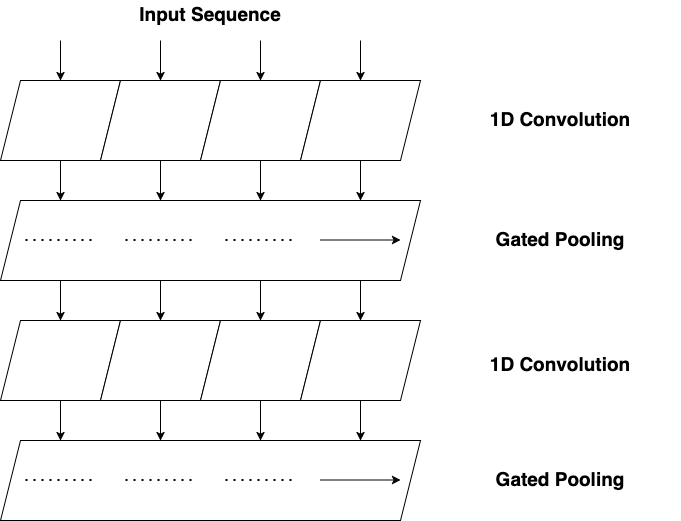
\includegraphics[width=0.48\textwidth]{QRNN_figure.png}
    \caption{Example of a QRNN architecture.}
\end{figure}

This figure higlights the two main components of QRNNs: the convolutional layer for feature extraction and the gated pooling mechanism for sequential processing.

In the convolutions layers, which are named as 1D Convolution in the figure, the input sequence is processed in parallel to extract local features.
Instead of processing tokens one-by-one like RNNs, QRNNs apply convolution filters to extract contextual features from multiple words simultaneously.
This step captures local dependencies, making it significantly faster than RNNs.

The next component after 1D Convolution is named as Gated Pooling in the figure, represent the gated pooling layers, which replace the traditional recurrent mechanism found in RNNs.
Instead of passing hidden states sequentially, gated pooling selectively retains or forgets information across time steps similar to LSTMs.
The dotted lines and rightward arrows indicate that pooling allows long-range dependencies to be retained without explicit recurrence.

Stacking multiple convolution + pooling layers allows QRNNs to capture both short-term and long-term dependencies effectively.

\pagebreak

\item[Problem 6:]  \hfill %Explain the role of subword information in language understanding.

Subword information plays a critical role in NLP by bridging the gap between character-based and word-based representations.
Instead of treating words as singular atomic units, subword models break words into smaller, meaningful components, 
which improves model performance in multiple linguistic and computational aspects.

By incorporating subwords, NLP models can handle rare and previously unseen words, significantly reducing errors in language modeling. 
This approach is particularly valuable for morphologically complex languages like Turkish, where words can take many different forms. 
Additionally, subword modeling helps reduce vocabulary size, making deep learning models more efficient without sacrificing expressiveness.
Another key advantage is its ability to enhance translation quality and tokenization, ensuring better alignment across different languages and writing systems. 
By leveraging subword information, models can achieve better generalization, improved computational efficiency, and enhanced performance in multilingual NLP tasks.

Different languages present unique challenges when processing words, especially those with rich morphology like Turkish. 
In such languages, words are often formed by adding multiple suffixes, which makes subword segmentation essential for better language modeling and machine translation.
In Turkish, a single root word can take on many different forms through suffixation. Consider the word "kitaplarımızdan" (from our books). 
The subword segmentation of this word would be 

\begin{center}
"kitap" + "lar" + "ımız" + "dan"
\end{center}

where each subword represents a meaningful morpheme.

\begin{itemize}
    \item kitap: root word, meaning "book"
    \item lar: plural suffix, books
    \item ımız: possessive suffix, (our books)
    \item dan: ablative case suffix, (from our books) 
\end{itemize}

In a standard word-based model, "kitaplarımızdan" would be treated as a completely separate token, making it hard to generalize across different word forms. 
However, by breaking it down into subwords, an NLP model can recognize morphological structures, improving performance in translation, text generation, and language modeling.

\pagebreak

\item[Problem 7:]  \hfill %Describe fully character-level neural machine translation.

Traditional neural machine translation models rely on word-based tokenization, which can lead to several issues. 
For instance, word-based models struggle with rare or unseen words. They also require large vocabularies to cover all possible words, 
since languages with many word forms like Turkish, Finnish, and Arabic require extensive vocabulary lists.
Lastly, tokenization at the word level may obscure relationships between words with similar roots.

Fully character-level neural machine translation on the other hand is an approach where translation models process text at the character level instead of using 
words or subwords as fundamental units. This method enables models to handle morphologically rich languages, spelling variations, and unknown words, making it 
particularly effective for languages with complex word structures.

Character-level neural machine translation follows the encoder-decoder structure, capturing fine-grained linguistic patterns.
The first step in character-level neural machine translation involves mapping each character in the input sentence to a character embedding.
These embeddings are passed through a CNN, which extract local patterns from the input text.
After extracting character-level features using a CNN, the output is processed through a highway network layer.
The highway network layer acts as a gating mechanism, deciding how much of the original character-level features should be retained or transformed.
This is mathematically formulated as 

\begin{center}
    $t = \sigma(W_T y + b_T)$

    $z = t \odot g(W_H y + b_H) + (1 - t) \odot y$
\end{center}

where $t$ is the transform gate that determines how much new information should be passed forward,
$y$ is the CNN output containing character-level features, $g$ is a non-linear activation function like ReLU,
and $z$ is the refined character-level representation that is sent to higher layers for processing.

The resulting feature representations are then passed to LSTM, which captures long-range dependencies in the sentence.
Finally, the LSTM output is fed into a softmax layer to generate the translation output.

\pagebreak

\item[Problem 8:]  \hfill %Explain byte pair encoding (BPE).

Byte Pair Encoding (BPE) is a subword tokenization method that efficiently processes text by iteratively merging frequently occurring character sequences. 
It is widely used in modern NLP models like GPT, and other Transformer-based architectures to handle rare words and reduce vocabulary size. 
Instead of relying on a fixed vocabulary of full words, BPE learns subword units dynamically, making it highly effective for morphologically rich languages and unseen words.

It begins with individual characters and progressively merges the most frequent adjacent characters to create subwords. 
This process is repeated until a predefined vocabulary size is reached. There are four main steps in the BPE algorithm.
As the first step, each word in the corpus is split into its basic character units. Then, as the next step, we identify the most frequent adjacent character pairs.
Thirdly, we replace the most frequent adjacent characters with a new subword unit.
Finally, we repeat the process until the desired vocabulary size is met.

Conside the Turkish word "evler" (houses). The BPE algorithm would tokenize it as follows:

\begin{center}
    $[e, v, l, e, r] \rightarrow [ev, l, e, r] \rightarrow [ev, le, r] \rightarrow [ev, ler]$
\end{center}

Instead of treating "evler" as a completely unique token, BPE identifies "ev" (house) and "ler" (plural suffix) as reusable subwords, 
allowing the model to efficiently process words like "evde" ([ev, de], at home), "evimiz" ([ev, im], my house), and "evlerden" ([ev, ler, den], from houses).

\pagebreak

\item[Problem 9:]  \hfill %Compare bottom-up and neural summarization.

Bottom-up summarization first extracts important content from the original text and then generates a summary based on the extracted key phrases and sentences.
This approach combines extractive and abstractive summarization, ensuring that the generated text remains factually consistent and informative.
In the extractive phase, the main job is content selection where the most important phrases and sentences are identified by attention mechanisms, 
TF-IDF, to score an rank importance before generating a summary.
In the abstractive phase, selected content is rewritten using an encoder-decoder model such as BART or Transformer-based architectures 
to ensure coherent, fluent, and factually grounded text generation.
This concept balances informativeness and conciseness by combining extraction and generation.

RL-based neural summarization, on the other hand, is an advanced approach that optimizes text generation using reward-based training. 
Unlike traditional models that use MLE, which trains models by maximizing word-level probabilities, RL trains models to optimize for long-term coherence, factuality, and human-preferred evaluation metrics.
The reason why RL-based neural summariation is that they cover up the downsides of MLE-based models.
Firstly, models are trained on selected summaries, but during inference, they must generate text from scratch, often leading to off-topic or incoherent outputs.
Secondly, MLE-based models optimize for word-level accuracy, but summarization is evaluated using sentence-level metrics, causing a mismatch between training and evaluation.
All these issues are adressed with a better training strategy to directly optimize for evaluation metrics, and with the inclusion of a reward function to 
guide the model towards generating more human-like summaries.
The summarization model is treated as an agent that generates text step by step, receiving reward signals based on the quality of the output.
A reward function evaluates summary coherence, factual correctness, and diversity, while policy gradient methods such as REINFORCE 
or SCST update the model to maximize expected rewards.
However, designing an effective reward function might be the challenge of neural summarization, along with the high computational resources needed for training.

\pagebreak

\item[Problem 10:]  \hfill %Discuss a method for handling irrelevant responses, generic outputs, repetition, and inconsistent persona in natural language generation.

\begin{enumerate}
    \item \textbf{Irrelevant Responses:} Seq2Seq models optimize for the likelihood of a response $P(T|S)$, which can lead to off-topic replies.
    With maximum mutual information (MMI) objective, we can introduce two additional terms as 

    \begin{center}
        argmax $P(T|S) - \lambda P(T)$
    \end{center}

    where $P(T|S)$ ensures the response logically connects with the input, and $P(T)$ penalizes generic responses by discouraging frequent outputs.
    With this objective function, we reduce off-topic responses by ensuring bidirectional relevance between the input and generated text while
    encouraging diversity by penalizing overused high-frequency responses.

    \item \textbf{Generic Outputs:} Seq2Seq models prefer safe and high-likelihood replies. This is mostly cuased by MLE optimizing for high-probability words, 
    making the model reluctant to generate richer, informative responses. To address this, we can ask model to upweight rare words in beam search to increases 
    the probability of less frequent terms, leading to more diverse responses. Another approach could be sampling-based decoding stragegies like top-k sampling to
    limit the word selection to the k-most probable tokens, and nucleus sampling to sample from the the set of words whose probabilities sum to p, 
    preventing the model from always selecting the highest probability word.

    \item \textbf{Repetition:} Seq2Seq models tend to repeat phrases within a response or generate similar responses across turns. This happens becuase of exposure bias, 
    where the model only sees ground-truth sequences during training but must generate new sequences at inference, and overfitting on high-frequency patterns in training data.
    To mitigate repetition, a simple fix could be blocking n-grams that have already been generated, preventing the model from repeating itself during beam search decoding.
    There are also more sophisticated methods like coverage mechanism that tracks previously attended words and reduces focus on already covered parts of the text. 
    Another approach is to introduce mutual information objectives that penalize duplicated phrases. Lastly, we can use reinforcement learning algorithm like SCST to 
    reward model for producing diverse responses.
    
    \item \textbf{Inconsistent Persona:} Standard Seq2Seq dialogue models lack personality memory, leading to contradictory or incoherent persona-related responses.
    Consider the scenario where a chatbot to simulate a travel assistant but fails to maintain a consistent persona throughout a conversation:

    \begin{itemize}
        \item User: "What’s your favorite city to visit?"
        \item Chatbot: "I love visiting Paris! The culture and food are amazing."
        \item User: "Have you ever been to France?"
        \item Chatbot: "No, I’ve never traveled to Europe."
        \item User: "Do you prefer Paris or London?"
        \item Chatbot: "I think London is my favorite city!"
    \end{itemize}

    This is problematic as the chatbot contradicts itself, claiming to love Paris but later stating it has never been to Europe.
    Furthermore, it switches preferences from Paris to London, indicating a lack of consistent persona. 
    
    To address this issue, early researchers back in 2016 proposed Persona-Embedded Seq2Seq Model, which encodes both user and AI persona embeddings into the dialogue model.
    This mechanism ensures that responses are conditioned on a persistent personality. Another approach named PersonaChat was proposed in 2018 by another researcher group.
    This is a dataset to train dialogue models by providing five explicit personality descriptions that the chatbot must adhere to throughout the conversation.
    Since the chatbot is conditioned on a fixed persona, this prevents contradictions and encourages personality-driven replies.

\end{enumerate}

\end{description}

\end{document}